\chapter{Introdução}
\section{Simulação}

A simulação é uma técnica que permite prever e visualizar o comportamento de sistemas reais a partir de modelos matemáticos. As aplicações da simulação abrangem diversos benefícios, tais como: a possibilidade de antever possíveis problemas ou comportamentos indesejáveis de um sistema, auxílio na tomada de decisão sem a necessidade de intervir no sistema real, facilidade na manipulação e alteração dos modelos, economia de recursos (físicos e financeiros) durante a tomada de decisões, dentre outros.

Para utilizar a simulação é necessário construir e analisar modelos que represente o sistema. Os modelos podem ser classificados de diferentes formas. Uma classificação pode ser considerada verificando a influência ou não de variáveis aleatórias no sistema. Os sistemas são ser representados por um modelo determinístico, quando estes podem ser considerado totalmente livre de aleatoriedade, ou estocásticos, quando estes consideram aleatoriedade.

Os modelos que descrevem o comportamento através do tempo podem ser classificados como contínuos e discretos no tempo. Nos modelos de estados contínuos, as variáveis de estados variam espontaneamente. Já nos modelos de estados discretos, as mudanças ocorrem em pontos específicos e descontínuos do tempo.

Este trabalho enfoca os modelos estocásticos e de estados discretos, uma vez que eles são os que melhor representam modelos de sistemas computacionais.

\subsection{Simulação Sequencial}

Um sistemas de simulação sequencial, onde uma única máquina executa toda a simulação, pode ser retratado como uma fila de eventos aguardando para serem tratados. Cada evento possui o seu tempo de execução, como pode ser visto na figura~\ref{fig:simul}, que deve ser obedecido para garantir consistência do resultado.

Neste modelo sequencial, o sistema responsável pela simulação retira o próximo evento da fila de execução para tratá-lo. Ao fim do processamento, um próximo evento é retirado da fila, e isto se repete até o final de lista de eventos futuros. O tratamento de um evento pode ou não resultar em dados que influenciem um processamento futuro.

\begin{figure}
  \centerline{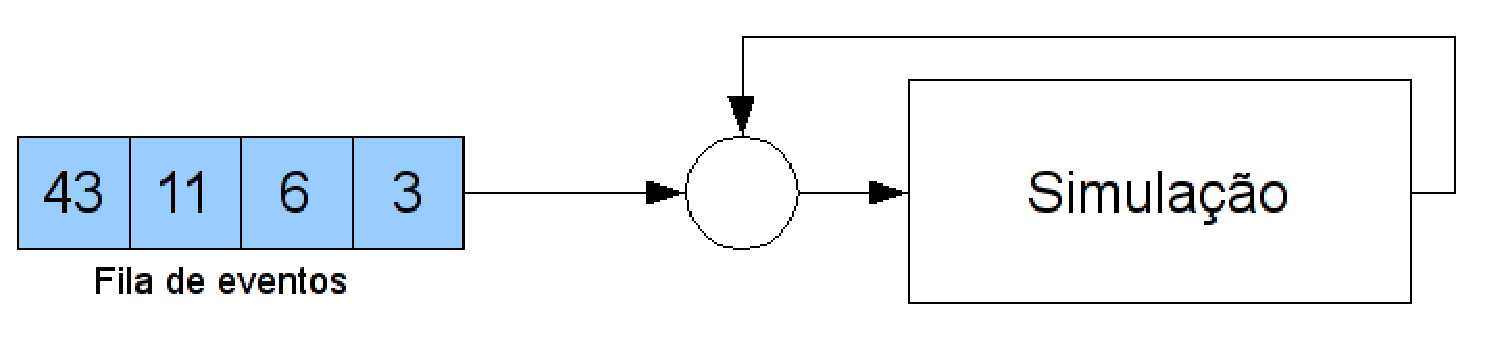
\includegraphics[scale=0.6]{simulacao.eps}}
  \caption{Simulação Sequencial.}
\label{fig:simul}
\end{figure}

\section{Simulação Distribuída}

A simulação é um processo que apresenta um custo computacional muito alto, tendo em vista a grande quantidade de dados que devem ser processados e a complexidade dos modelos matemáticos empregados. Esses fatores em conjunto podem encarecer computacionalmente o sistema, levando à ineficiência da simulação.

Uma das formas encontradas para se solucionar estes problemas foi dividir o tratamento dos diversos eventos entre vários processadores de uma mesma máquina paralela ou sobre um sistema distribuído, dando origem assim à Simulação Distribuída.

Distribuindo os eventos, reduz-se o tempo gasto pelos programas de simulação, mas, em contrapartida, novas situações necessitam de observação devido às características deste tipo de aplicação. É preciso sanar os problemas com a sincronização dos processos, sobrecarga da rede de comunicação, necessidade de balanceamento de carga do sistema, dentre outros.



\section{Objetivo}
\section{Organização Do Documento}

O segundo capítulo traz uma abordagem introdutória à simulação distribuída de eventos discretos e descreve os princípios de dois protocolos utilizados para sincronização de simulação distribuída.

O Terceiro capítulo aprofunda-se na proposta do projeto, apresentando a arquitetura básica do \textit{middleware} de comunicação que propõe proporcionar mobilidade aos processos lógicos no sistema de simulação distribuída. 

Os capítulos quatro e cinco apresentam, consecutivamente, a arquitetura interna do \textit{middleware} de comunicação e a arquitetura de um micro-\textit{framework} desenvolvido para demonstrar o funcionamento do \textit{middleware} de comunicação.

Por fim o capítulo sete traz alguns detalhes de implementação do \textit{middleware} proposto que o autor julgou conveniente descrever, seguido pela conclusão, compondo o oitavo capítulo.
